% Options for packages loaded elsewhere
\PassOptionsToPackage{unicode}{hyperref}
\PassOptionsToPackage{hyphens}{url}
\PassOptionsToPackage{dvipsnames,svgnames,x11names}{xcolor}
%
\documentclass[
  letterpaper,
  DIV=11,
  numbers=noendperiod]{scrartcl}

\usepackage{amsmath,amssymb}
\usepackage{iftex}
\ifPDFTeX
  \usepackage[T1]{fontenc}
  \usepackage[utf8]{inputenc}
  \usepackage{textcomp} % provide euro and other symbols
\else % if luatex or xetex
  \usepackage{unicode-math}
  \defaultfontfeatures{Scale=MatchLowercase}
  \defaultfontfeatures[\rmfamily]{Ligatures=TeX,Scale=1}
\fi
\usepackage{lmodern}
\ifPDFTeX\else  
    % xetex/luatex font selection
\fi
% Use upquote if available, for straight quotes in verbatim environments
\IfFileExists{upquote.sty}{\usepackage{upquote}}{}
\IfFileExists{microtype.sty}{% use microtype if available
  \usepackage[]{microtype}
  \UseMicrotypeSet[protrusion]{basicmath} % disable protrusion for tt fonts
}{}
\makeatletter
\@ifundefined{KOMAClassName}{% if non-KOMA class
  \IfFileExists{parskip.sty}{%
    \usepackage{parskip}
  }{% else
    \setlength{\parindent}{0pt}
    \setlength{\parskip}{6pt plus 2pt minus 1pt}}
}{% if KOMA class
  \KOMAoptions{parskip=half}}
\makeatother
\usepackage{xcolor}
\setlength{\emergencystretch}{3em} % prevent overfull lines
\setcounter{secnumdepth}{-\maxdimen} % remove section numbering
% Make \paragraph and \subparagraph free-standing
\ifx\paragraph\undefined\else
  \let\oldparagraph\paragraph
  \renewcommand{\paragraph}[1]{\oldparagraph{#1}\mbox{}}
\fi
\ifx\subparagraph\undefined\else
  \let\oldsubparagraph\subparagraph
  \renewcommand{\subparagraph}[1]{\oldsubparagraph{#1}\mbox{}}
\fi

\usepackage{color}
\usepackage{fancyvrb}
\newcommand{\VerbBar}{|}
\newcommand{\VERB}{\Verb[commandchars=\\\{\}]}
\DefineVerbatimEnvironment{Highlighting}{Verbatim}{commandchars=\\\{\}}
% Add ',fontsize=\small' for more characters per line
\usepackage{framed}
\definecolor{shadecolor}{RGB}{241,243,245}
\newenvironment{Shaded}{\begin{snugshade}}{\end{snugshade}}
\newcommand{\AlertTok}[1]{\textcolor[rgb]{0.68,0.00,0.00}{#1}}
\newcommand{\AnnotationTok}[1]{\textcolor[rgb]{0.37,0.37,0.37}{#1}}
\newcommand{\AttributeTok}[1]{\textcolor[rgb]{0.40,0.45,0.13}{#1}}
\newcommand{\BaseNTok}[1]{\textcolor[rgb]{0.68,0.00,0.00}{#1}}
\newcommand{\BuiltInTok}[1]{\textcolor[rgb]{0.00,0.23,0.31}{#1}}
\newcommand{\CharTok}[1]{\textcolor[rgb]{0.13,0.47,0.30}{#1}}
\newcommand{\CommentTok}[1]{\textcolor[rgb]{0.37,0.37,0.37}{#1}}
\newcommand{\CommentVarTok}[1]{\textcolor[rgb]{0.37,0.37,0.37}{\textit{#1}}}
\newcommand{\ConstantTok}[1]{\textcolor[rgb]{0.56,0.35,0.01}{#1}}
\newcommand{\ControlFlowTok}[1]{\textcolor[rgb]{0.00,0.23,0.31}{#1}}
\newcommand{\DataTypeTok}[1]{\textcolor[rgb]{0.68,0.00,0.00}{#1}}
\newcommand{\DecValTok}[1]{\textcolor[rgb]{0.68,0.00,0.00}{#1}}
\newcommand{\DocumentationTok}[1]{\textcolor[rgb]{0.37,0.37,0.37}{\textit{#1}}}
\newcommand{\ErrorTok}[1]{\textcolor[rgb]{0.68,0.00,0.00}{#1}}
\newcommand{\ExtensionTok}[1]{\textcolor[rgb]{0.00,0.23,0.31}{#1}}
\newcommand{\FloatTok}[1]{\textcolor[rgb]{0.68,0.00,0.00}{#1}}
\newcommand{\FunctionTok}[1]{\textcolor[rgb]{0.28,0.35,0.67}{#1}}
\newcommand{\ImportTok}[1]{\textcolor[rgb]{0.00,0.46,0.62}{#1}}
\newcommand{\InformationTok}[1]{\textcolor[rgb]{0.37,0.37,0.37}{#1}}
\newcommand{\KeywordTok}[1]{\textcolor[rgb]{0.00,0.23,0.31}{#1}}
\newcommand{\NormalTok}[1]{\textcolor[rgb]{0.00,0.23,0.31}{#1}}
\newcommand{\OperatorTok}[1]{\textcolor[rgb]{0.37,0.37,0.37}{#1}}
\newcommand{\OtherTok}[1]{\textcolor[rgb]{0.00,0.23,0.31}{#1}}
\newcommand{\PreprocessorTok}[1]{\textcolor[rgb]{0.68,0.00,0.00}{#1}}
\newcommand{\RegionMarkerTok}[1]{\textcolor[rgb]{0.00,0.23,0.31}{#1}}
\newcommand{\SpecialCharTok}[1]{\textcolor[rgb]{0.37,0.37,0.37}{#1}}
\newcommand{\SpecialStringTok}[1]{\textcolor[rgb]{0.13,0.47,0.30}{#1}}
\newcommand{\StringTok}[1]{\textcolor[rgb]{0.13,0.47,0.30}{#1}}
\newcommand{\VariableTok}[1]{\textcolor[rgb]{0.07,0.07,0.07}{#1}}
\newcommand{\VerbatimStringTok}[1]{\textcolor[rgb]{0.13,0.47,0.30}{#1}}
\newcommand{\WarningTok}[1]{\textcolor[rgb]{0.37,0.37,0.37}{\textit{#1}}}

\providecommand{\tightlist}{%
  \setlength{\itemsep}{0pt}\setlength{\parskip}{0pt}}\usepackage{longtable,booktabs,array}
\usepackage{calc} % for calculating minipage widths
% Correct order of tables after \paragraph or \subparagraph
\usepackage{etoolbox}
\makeatletter
\patchcmd\longtable{\par}{\if@noskipsec\mbox{}\fi\par}{}{}
\makeatother
% Allow footnotes in longtable head/foot
\IfFileExists{footnotehyper.sty}{\usepackage{footnotehyper}}{\usepackage{footnote}}
\makesavenoteenv{longtable}
\usepackage{graphicx}
\makeatletter
\def\maxwidth{\ifdim\Gin@nat@width>\linewidth\linewidth\else\Gin@nat@width\fi}
\def\maxheight{\ifdim\Gin@nat@height>\textheight\textheight\else\Gin@nat@height\fi}
\makeatother
% Scale images if necessary, so that they will not overflow the page
% margins by default, and it is still possible to overwrite the defaults
% using explicit options in \includegraphics[width, height, ...]{}
\setkeys{Gin}{width=\maxwidth,height=\maxheight,keepaspectratio}
% Set default figure placement to htbp
\makeatletter
\def\fps@figure{htbp}
\makeatother

\usepackage{booktabs}
\usepackage{caption}
\usepackage{longtable}
\usepackage{colortbl}
\usepackage{array}
\usepackage{multirow}
\usepackage{wrapfig}
\usepackage{float}
\usepackage{pdflscape}
\usepackage{tabu}
\usepackage{threeparttable}
\usepackage{threeparttablex}
\usepackage[normalem]{ulem}
\usepackage{makecell}
\usepackage{xcolor}
\KOMAoption{captions}{tableheading}
\makeatletter
\makeatother
\makeatletter
\makeatother
\makeatletter
\@ifpackageloaded{caption}{}{\usepackage{caption}}
\AtBeginDocument{%
\ifdefined\contentsname
  \renewcommand*\contentsname{Table of contents}
\else
  \newcommand\contentsname{Table of contents}
\fi
\ifdefined\listfigurename
  \renewcommand*\listfigurename{List of Figures}
\else
  \newcommand\listfigurename{List of Figures}
\fi
\ifdefined\listtablename
  \renewcommand*\listtablename{List of Tables}
\else
  \newcommand\listtablename{List of Tables}
\fi
\ifdefined\figurename
  \renewcommand*\figurename{Figure}
\else
  \newcommand\figurename{Figure}
\fi
\ifdefined\tablename
  \renewcommand*\tablename{Table}
\else
  \newcommand\tablename{Table}
\fi
}
\@ifpackageloaded{float}{}{\usepackage{float}}
\floatstyle{ruled}
\@ifundefined{c@chapter}{\newfloat{codelisting}{h}{lop}}{\newfloat{codelisting}{h}{lop}[chapter]}
\floatname{codelisting}{Listing}
\newcommand*\listoflistings{\listof{codelisting}{List of Listings}}
\makeatother
\makeatletter
\@ifpackageloaded{caption}{}{\usepackage{caption}}
\@ifpackageloaded{subcaption}{}{\usepackage{subcaption}}
\makeatother
\makeatletter
\@ifpackageloaded{tcolorbox}{}{\usepackage[skins,breakable]{tcolorbox}}
\makeatother
\makeatletter
\@ifundefined{shadecolor}{\definecolor{shadecolor}{rgb}{.97, .97, .97}}
\makeatother
\makeatletter
\makeatother
\makeatletter
\makeatother
\ifLuaTeX
  \usepackage{selnolig}  % disable illegal ligatures
\fi
\IfFileExists{bookmark.sty}{\usepackage{bookmark}}{\usepackage{hyperref}}
\IfFileExists{xurl.sty}{\usepackage{xurl}}{} % add URL line breaks if available
\urlstyle{same} % disable monospaced font for URLs
\hypersetup{
  colorlinks=true,
  linkcolor={blue},
  filecolor={Maroon},
  citecolor={Blue},
  urlcolor={Blue},
  pdfcreator={LaTeX via pandoc}}

\author{}
\date{}

\begin{document}
\ifdefined\Shaded\renewenvironment{Shaded}{\begin{tcolorbox}[frame hidden, interior hidden, boxrule=0pt, sharp corners, enhanced, borderline west={3pt}{0pt}{shadecolor}, breakable]}{\end{tcolorbox}}\fi

\begin{Shaded}
\begin{Highlighting}[]
\FunctionTok{library}\NormalTok{(tidyverse)}
\end{Highlighting}
\end{Shaded}

\begin{verbatim}
-- Attaching core tidyverse packages ------------------------ tidyverse 2.0.0 --
v dplyr     1.1.4     v readr     2.1.4
v forcats   1.0.0     v stringr   1.5.1
v ggplot2   3.4.4     v tibble    3.2.1
v lubridate 1.9.3     v tidyr     1.3.0
v purrr     1.0.2     
-- Conflicts ------------------------------------------ tidyverse_conflicts() --
x dplyr::filter() masks stats::filter()
x dplyr::lag()    masks stats::lag()
i Use the conflicted package (<http://conflicted.r-lib.org/>) to force all conflicts to become errors
\end{verbatim}

\begin{Shaded}
\begin{Highlighting}[]
\FunctionTok{library}\NormalTok{(gt)}
\CommentTok{\#library(knitr)}
\CommentTok{\#library(kableExtra)}
\CommentTok{\#library(gtExtras)}
\end{Highlighting}
\end{Shaded}

\begin{Shaded}
\begin{Highlighting}[]
\FunctionTok{gt}\NormalTok{(}\FunctionTok{head}\NormalTok{(iris)) }\SpecialCharTok{|\textgreater{}} 
  \FunctionTok{tab\_source\_note}\NormalTok{(}\AttributeTok{source\_note =} \FunctionTok{md}\NormalTok{(}\StringTok{"Data Source: Powell \& Thyne (2011)"}\NormalTok{))}
\end{Highlighting}
\end{Shaded}

\setlength{\LTpost}{0mm}
\begin{longtable*}{rrrrc}
\toprule
Sepal.Length & Sepal.Width & Petal.Length & Petal.Width & Species \\ 
\midrule\addlinespace[2.5pt]
5.1 & 3.5 & 1.4 & 0.2 & setosa \\ 
4.9 & 3.0 & 1.4 & 0.2 & setosa \\ 
4.7 & 3.2 & 1.3 & 0.2 & setosa \\ 
4.6 & 3.1 & 1.5 & 0.2 & setosa \\ 
5.0 & 3.6 & 1.4 & 0.2 & setosa \\ 
5.4 & 3.9 & 1.7 & 0.4 & setosa \\ 
\bottomrule
\end{longtable*}
\begin{minipage}{\linewidth}
Data Source: Powell \& Thyne (2011)\\
\end{minipage}

\begin{Shaded}
\begin{Highlighting}[]
\NormalTok{mtcars }\SpecialCharTok{|\textgreater{}} 
  \FunctionTok{gt}\NormalTok{() }\SpecialCharTok{|\textgreater{}}  
  \FunctionTok{cols\_label}\NormalTok{(}\AttributeTok{mpg =} \StringTok{"miles per gal"}\NormalTok{,}
             \AttributeTok{cyl =} \StringTok{"Number of cylinders"}\NormalTok{,}
             \AttributeTok{disp =} \StringTok{"Displacement (cu.in.)"}\NormalTok{,}
             \AttributeTok{hp =} \StringTok{"Gross horsepower"}
\NormalTok{             ) }
\end{Highlighting}
\end{Shaded}

\begin{longtable*}{rrrrrrrrrrr}
\toprule
miles per gal & Number of cylinders & Displacement (cu.in.) & Gross horsepower & drat & wt & qsec & vs & am & gear & carb \\ 
\midrule\addlinespace[2.5pt]
21.0 & 6 & 160.0 & 110 & 3.90 & 2.620 & 16.46 & 0 & 1 & 4 & 4 \\ 
21.0 & 6 & 160.0 & 110 & 3.90 & 2.875 & 17.02 & 0 & 1 & 4 & 4 \\ 
22.8 & 4 & 108.0 & 93 & 3.85 & 2.320 & 18.61 & 1 & 1 & 4 & 1 \\ 
21.4 & 6 & 258.0 & 110 & 3.08 & 3.215 & 19.44 & 1 & 0 & 3 & 1 \\ 
18.7 & 8 & 360.0 & 175 & 3.15 & 3.440 & 17.02 & 0 & 0 & 3 & 2 \\ 
18.1 & 6 & 225.0 & 105 & 2.76 & 3.460 & 20.22 & 1 & 0 & 3 & 1 \\ 
14.3 & 8 & 360.0 & 245 & 3.21 & 3.570 & 15.84 & 0 & 0 & 3 & 4 \\ 
24.4 & 4 & 146.7 & 62 & 3.69 & 3.190 & 20.00 & 1 & 0 & 4 & 2 \\ 
22.8 & 4 & 140.8 & 95 & 3.92 & 3.150 & 22.90 & 1 & 0 & 4 & 2 \\ 
19.2 & 6 & 167.6 & 123 & 3.92 & 3.440 & 18.30 & 1 & 0 & 4 & 4 \\ 
17.8 & 6 & 167.6 & 123 & 3.92 & 3.440 & 18.90 & 1 & 0 & 4 & 4 \\ 
16.4 & 8 & 275.8 & 180 & 3.07 & 4.070 & 17.40 & 0 & 0 & 3 & 3 \\ 
17.3 & 8 & 275.8 & 180 & 3.07 & 3.730 & 17.60 & 0 & 0 & 3 & 3 \\ 
15.2 & 8 & 275.8 & 180 & 3.07 & 3.780 & 18.00 & 0 & 0 & 3 & 3 \\ 
10.4 & 8 & 472.0 & 205 & 2.93 & 5.250 & 17.98 & 0 & 0 & 3 & 4 \\ 
10.4 & 8 & 460.0 & 215 & 3.00 & 5.424 & 17.82 & 0 & 0 & 3 & 4 \\ 
14.7 & 8 & 440.0 & 230 & 3.23 & 5.345 & 17.42 & 0 & 0 & 3 & 4 \\ 
32.4 & 4 & 78.7 & 66 & 4.08 & 2.200 & 19.47 & 1 & 1 & 4 & 1 \\ 
30.4 & 4 & 75.7 & 52 & 4.93 & 1.615 & 18.52 & 1 & 1 & 4 & 2 \\ 
33.9 & 4 & 71.1 & 65 & 4.22 & 1.835 & 19.90 & 1 & 1 & 4 & 1 \\ 
21.5 & 4 & 120.1 & 97 & 3.70 & 2.465 & 20.01 & 1 & 0 & 3 & 1 \\ 
15.5 & 8 & 318.0 & 150 & 2.76 & 3.520 & 16.87 & 0 & 0 & 3 & 2 \\ 
15.2 & 8 & 304.0 & 150 & 3.15 & 3.435 & 17.30 & 0 & 0 & 3 & 2 \\ 
13.3 & 8 & 350.0 & 245 & 3.73 & 3.840 & 15.41 & 0 & 0 & 3 & 4 \\ 
19.2 & 8 & 400.0 & 175 & 3.08 & 3.845 & 17.05 & 0 & 0 & 3 & 2 \\ 
27.3 & 4 & 79.0 & 66 & 4.08 & 1.935 & 18.90 & 1 & 1 & 4 & 1 \\ 
26.0 & 4 & 120.3 & 91 & 4.43 & 2.140 & 16.70 & 0 & 1 & 5 & 2 \\ 
30.4 & 4 & 95.1 & 113 & 3.77 & 1.513 & 16.90 & 1 & 1 & 5 & 2 \\ 
15.8 & 8 & 351.0 & 264 & 4.22 & 3.170 & 14.50 & 0 & 1 & 5 & 4 \\ 
19.7 & 6 & 145.0 & 175 & 3.62 & 2.770 & 15.50 & 0 & 1 & 5 & 6 \\ 
15.0 & 8 & 301.0 & 335 & 3.54 & 3.570 & 14.60 & 0 & 1 & 5 & 8 \\ 
21.4 & 4 & 121.0 & 109 & 4.11 & 2.780 & 18.60 & 1 & 1 & 4 & 2 \\ 
\bottomrule
\end{longtable*}

\begin{Shaded}
\begin{Highlighting}[]
\CommentTok{\# |\textgreater{} }
\CommentTok{\#   as\_latex()}
\end{Highlighting}
\end{Shaded}

\begin{Shaded}
\begin{Highlighting}[]
\NormalTok{mtcars }\SpecialCharTok{\%\textgreater{}\%} 
  \FunctionTok{select}\NormalTok{(}\DecValTok{1}\SpecialCharTok{:}\DecValTok{2}\NormalTok{) }\SpecialCharTok{|\textgreater{}} 
\NormalTok{  knitr}\SpecialCharTok{::}\FunctionTok{kable}\NormalTok{(}\AttributeTok{col.names =} \FunctionTok{c}\NormalTok{(}\StringTok{"miles per gal"}\NormalTok{, }\StringTok{"Number of cylinders"}\NormalTok{))}
\end{Highlighting}
\end{Shaded}

\hypertarget{tbl-1}{}
\begin{longtable}[]{@{}
  >{\raggedright\arraybackslash}p{(\columnwidth - 4\tabcolsep) * \real{0.2000}}
  >{\raggedleft\arraybackslash}p{(\columnwidth - 4\tabcolsep) * \real{0.3500}}
  >{\raggedleft\arraybackslash}p{(\columnwidth - 4\tabcolsep) * \real{0.3500}}@{}}
\caption{\label{tbl-1}mtcars}\tabularnewline
\toprule\noalign{}
\begin{minipage}[b]{\linewidth}\raggedright
\end{minipage} & \begin{minipage}[b]{\linewidth}\raggedleft
miles per gal
\end{minipage} & \begin{minipage}[b]{\linewidth}\raggedleft
Number of cylinders
\end{minipage} \\
\midrule\noalign{}
\endfirsthead
\toprule\noalign{}
\begin{minipage}[b]{\linewidth}\raggedright
\end{minipage} & \begin{minipage}[b]{\linewidth}\raggedleft
miles per gal
\end{minipage} & \begin{minipage}[b]{\linewidth}\raggedleft
Number of cylinders
\end{minipage} \\
\midrule\noalign{}
\endhead
\bottomrule\noalign{}
\endlastfoot
Mazda RX4 & 21.0 & 6 \\
Mazda RX4 Wag & 21.0 & 6 \\
Datsun 710 & 22.8 & 4 \\
Hornet 4 Drive & 21.4 & 6 \\
Hornet Sportabout & 18.7 & 8 \\
Valiant & 18.1 & 6 \\
Duster 360 & 14.3 & 8 \\
Merc 240D & 24.4 & 4 \\
Merc 230 & 22.8 & 4 \\
Merc 280 & 19.2 & 6 \\
Merc 280C & 17.8 & 6 \\
Merc 450SE & 16.4 & 8 \\
Merc 450SL & 17.3 & 8 \\
Merc 450SLC & 15.2 & 8 \\
Cadillac Fleetwood & 10.4 & 8 \\
Lincoln Continental & 10.4 & 8 \\
Chrysler Imperial & 14.7 & 8 \\
Fiat 128 & 32.4 & 4 \\
Honda Civic & 30.4 & 4 \\
Toyota Corolla & 33.9 & 4 \\
Toyota Corona & 21.5 & 4 \\
Dodge Challenger & 15.5 & 8 \\
AMC Javelin & 15.2 & 8 \\
Camaro Z28 & 13.3 & 8 \\
Pontiac Firebird & 19.2 & 8 \\
Fiat X1-9 & 27.3 & 4 \\
Porsche 914-2 & 26.0 & 4 \\
Lotus Europa & 30.4 & 4 \\
Ford Pantera L & 15.8 & 8 \\
Ferrari Dino & 19.7 & 6 \\
Maserati Bora & 15.0 & 8 \\
Volvo 142E & 21.4 & 4 \\
\end{longtable}

\begin{Shaded}
\begin{Highlighting}[]
\NormalTok{mtcars }\SpecialCharTok{|\textgreater{}} 
  \FunctionTok{select}\NormalTok{(}\DecValTok{1}\SpecialCharTok{:}\DecValTok{2}\NormalTok{) }\SpecialCharTok{|\textgreater{}} 
\NormalTok{  knitr}\SpecialCharTok{::}\FunctionTok{kable}\NormalTok{()}
\end{Highlighting}
\end{Shaded}

\begin{table}

\caption{\textbf{?(caption)}}\begin{minipage}[t]{\linewidth}

{\centering 

\begin{longtable}[]{@{}
  >{\raggedright\arraybackslash}p{(\columnwidth - 4\tabcolsep) * \real{0.2000}}
  >{\raggedleft\arraybackslash}p{(\columnwidth - 4\tabcolsep) * \real{0.3000}}
  >{\raggedleft\arraybackslash}p{(\columnwidth - 4\tabcolsep) * \real{0.3000}}@{}}
\toprule\noalign{}
\begin{minipage}[b]{\linewidth}\raggedright
\end{minipage} & \begin{minipage}[b]{\linewidth}\raggedleft
mpg
\end{minipage} & \begin{minipage}[b]{\linewidth}\raggedleft
cyl
\end{minipage} \\
\midrule\noalign{}
\endhead
\bottomrule\noalign{}
\endlastfoot
Mazda RX4 & 21.0 & 6 \\
Mazda RX4 Wag & 21.0 & 6 \\
Datsun 710 & 22.8 & 4 \\
Hornet 4 Drive & 21.4 & 6 \\
Hornet Sportabout & 18.7 & 8 \\
Valiant & 18.1 & 6 \\
Duster 360 & 14.3 & 8 \\
Merc 240D & 24.4 & 4 \\
Merc 230 & 22.8 & 4 \\
Merc 280 & 19.2 & 6 \\
Merc 280C & 17.8 & 6 \\
Merc 450SE & 16.4 & 8 \\
Merc 450SL & 17.3 & 8 \\
Merc 450SLC & 15.2 & 8 \\
Cadillac Fleetwood & 10.4 & 8 \\
Lincoln Continental & 10.4 & 8 \\
Chrysler Imperial & 14.7 & 8 \\
Fiat 128 & 32.4 & 4 \\
Honda Civic & 30.4 & 4 \\
Toyota Corolla & 33.9 & 4 \\
Toyota Corona & 21.5 & 4 \\
Dodge Challenger & 15.5 & 8 \\
AMC Javelin & 15.2 & 8 \\
Camaro Z28 & 13.3 & 8 \\
Pontiac Firebird & 19.2 & 8 \\
Fiat X1-9 & 27.3 & 4 \\
Porsche 914-2 & 26.0 & 4 \\
Lotus Europa & 30.4 & 4 \\
Ford Pantera L & 15.8 & 8 \\
Ferrari Dino & 19.7 & 6 \\
Maserati Bora & 15.0 & 8 \\
Volvo 142E & 21.4 & 4 \\
\end{longtable}

}

\end{minipage}%

\end{table}

\begin{Shaded}
\begin{Highlighting}[]
\NormalTok{gtcars }\SpecialCharTok{|\textgreater{}}
  \FunctionTok{select}\NormalTok{(mfr, model, msrp) }\SpecialCharTok{|\textgreater{}}
  \FunctionTok{slice}\NormalTok{(}\DecValTok{1}\SpecialCharTok{:}\DecValTok{5}\NormalTok{) }\SpecialCharTok{|\textgreater{}}
  \FunctionTok{gt}\NormalTok{()}
\end{Highlighting}
\end{Shaded}

\begin{table}

\caption{\label{tbl-gtcars}\textbf{?(caption)}}\begin{minipage}[t]{\linewidth}
\subcaption{\label{tbl-gtcars-1}}

{\centering 

\begin{longtable*}{llr}
\toprule
mfr & model & msrp \\ 
\midrule\addlinespace[2.5pt]
Ford & GT & 447000 \\ 
Ferrari & 458 Speciale & 291744 \\ 
Ferrari & 458 Spider & 263553 \\ 
Ferrari & 458 Italia & 233509 \\ 
Ferrari & 488 GTB & 245400 \\ 
\bottomrule
\end{longtable*}

}

\end{minipage}%

\end{table}

\begin{Shaded}
\begin{Highlighting}[]
\NormalTok{islands\_tbl }\OtherTok{\textless{}{-}} 
  \FunctionTok{tibble}\NormalTok{(}
    \AttributeTok{name =} \FunctionTok{names}\NormalTok{(islands),}
    \AttributeTok{size =}\NormalTok{ islands}
\NormalTok{  ) }\SpecialCharTok{\%\textgreater{}\%}
  \FunctionTok{arrange}\NormalTok{(}\FunctionTok{desc}\NormalTok{(size)) }\SpecialCharTok{\%\textgreater{}\%}
  \FunctionTok{slice}\NormalTok{(}\DecValTok{1}\SpecialCharTok{:}\DecValTok{10}\NormalTok{)}


\FunctionTok{gt}\NormalTok{(islands\_tbl) }\SpecialCharTok{\%\textgreater{}\%} 
  \FunctionTok{gtsave}\NormalTok{(}\StringTok{\textquotesingle{}islands.png\textquotesingle{}}\NormalTok{)}

\NormalTok{knitr}\SpecialCharTok{::}\FunctionTok{include\_graphics}\NormalTok{(}\StringTok{\textquotesingle{}islands.png\textquotesingle{}}\NormalTok{)}
\end{Highlighting}
\end{Shaded}

\begin{table}

\caption{\textbf{?(caption)}}\begin{minipage}[t]{\linewidth}

{\centering 

\raisebox{-\height}{

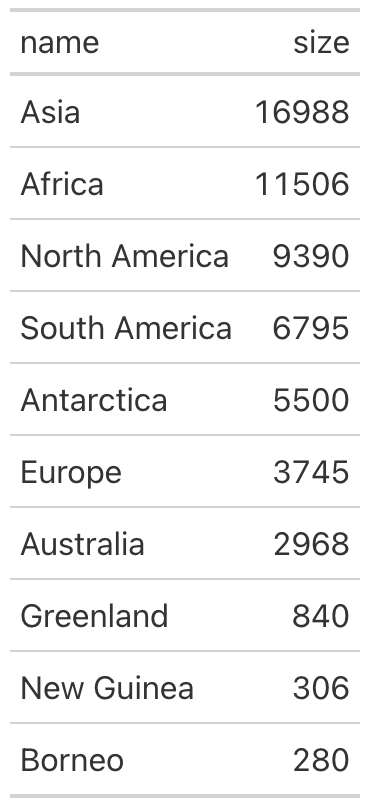
\includegraphics[width=1.23in,height=\textheight]{islands.png}

}

}

\end{minipage}%

\end{table}

\begin{Shaded}
\begin{Highlighting}[]
\FunctionTok{library}\NormalTok{(kableExtra)}
\end{Highlighting}
\end{Shaded}

\begin{verbatim}
Registered S3 method overwritten by 'webshot':
  method        from    
  print.webshot webshot2
\end{verbatim}

\begin{verbatim}

Attaching package: 'kableExtra'
\end{verbatim}

\begin{verbatim}
The following object is masked from 'package:dplyr':

    group_rows
\end{verbatim}

\begin{Shaded}
\begin{Highlighting}[]
\NormalTok{mtcars[}\DecValTok{1}\SpecialCharTok{:}\DecValTok{8}\NormalTok{,}\DecValTok{1}\SpecialCharTok{:}\DecValTok{3}\NormalTok{] }\SpecialCharTok{|\textgreater{}} 
  \FunctionTok{kable}\NormalTok{(}\StringTok{"latex"}\NormalTok{, }\AttributeTok{booktabs =}\NormalTok{ T) }\SpecialCharTok{\%\textgreater{}\%}
  \FunctionTok{kable\_styling}\NormalTok{(}\AttributeTok{latex\_options =} \StringTok{"striped"}\NormalTok{) }\SpecialCharTok{|\textgreater{}} 
  \FunctionTok{collapse\_rows}\NormalTok{(}\AttributeTok{latex\_hline =} \StringTok{"linespace"}\NormalTok{,}
                \AttributeTok{longtable\_clean\_cut =}\NormalTok{ T) }\SpecialCharTok{|\textgreater{}} 
  \FunctionTok{column\_spec}\NormalTok{(}\AttributeTok{column =} \DecValTok{1}\SpecialCharTok{:}\DecValTok{4}\NormalTok{,}\AttributeTok{width =} \StringTok{"3cm"}\NormalTok{) }\SpecialCharTok{|\textgreater{}} 
  \FunctionTok{footnote}\NormalTok{(}\AttributeTok{general =} \StringTok{""}\NormalTok{,}
           \AttributeTok{general\_title =} \StringTok{"test"}\NormalTok{)}
\end{Highlighting}
\end{Shaded}

\begin{verbatim}
Usually it is recommended to use column_spec before collapse_rows, especially in LaTeX, to get a desired result. 
\end{verbatim}

\hypertarget{tbl-7}{}
\begin{table}
\caption{\label{tbl-7}This is a kable table }\tabularnewline

\centering
\begin{tabular}{>{\raggedright\arraybackslash}p{3cm}>{\raggedleft\arraybackslash}p{3cm}>{\raggedleft\arraybackslash}p{3cm}>{\raggedleft\arraybackslash}p{3cm}}
\toprule
  & mpg & cyl & disp\\
\midrule
\cellcolor{gray!6}{Mazda RX4} & \cellcolor{gray!6}{21.0} & \cellcolor{gray!6}{6} & \cellcolor{gray!6}{160.0}\\
\addlinespace
Mazda RX4 Wag & 21.0 & 6 & 160.0\\
\addlinespace
\cellcolor{gray!6}{Datsun 710} & \cellcolor{gray!6}{22.8} & \cellcolor{gray!6}{4} & \cellcolor{gray!6}{108.0}\\
\addlinespace
Hornet 4 Drive & 21.4 & 6 & 258.0\\
\addlinespace
\cellcolor{gray!6}{Hornet Sportabout} & \cellcolor{gray!6}{18.7} & \cellcolor{gray!6}{8} & \cellcolor{gray!6}{360.0}\\
\addlinespace
Valiant & 18.1 & 6 & 225.0\\
\addlinespace
\cellcolor{gray!6}{Duster 360} & \cellcolor{gray!6}{14.3} & \cellcolor{gray!6}{8} & \cellcolor{gray!6}{360.0}\\
\addlinespace
Merc 240D & 24.4 & 4 & 146.7\\
\bottomrule
\multicolumn{4}{l}{\rule{0pt}{1em}\textit{test}}\\
\multicolumn{4}{l}{\rule{0pt}{1em}}\\
\end{tabular}
\end{table}



\end{document}
